\section{Architecture}

\begin{figure}[htbp]
   \centerline{
   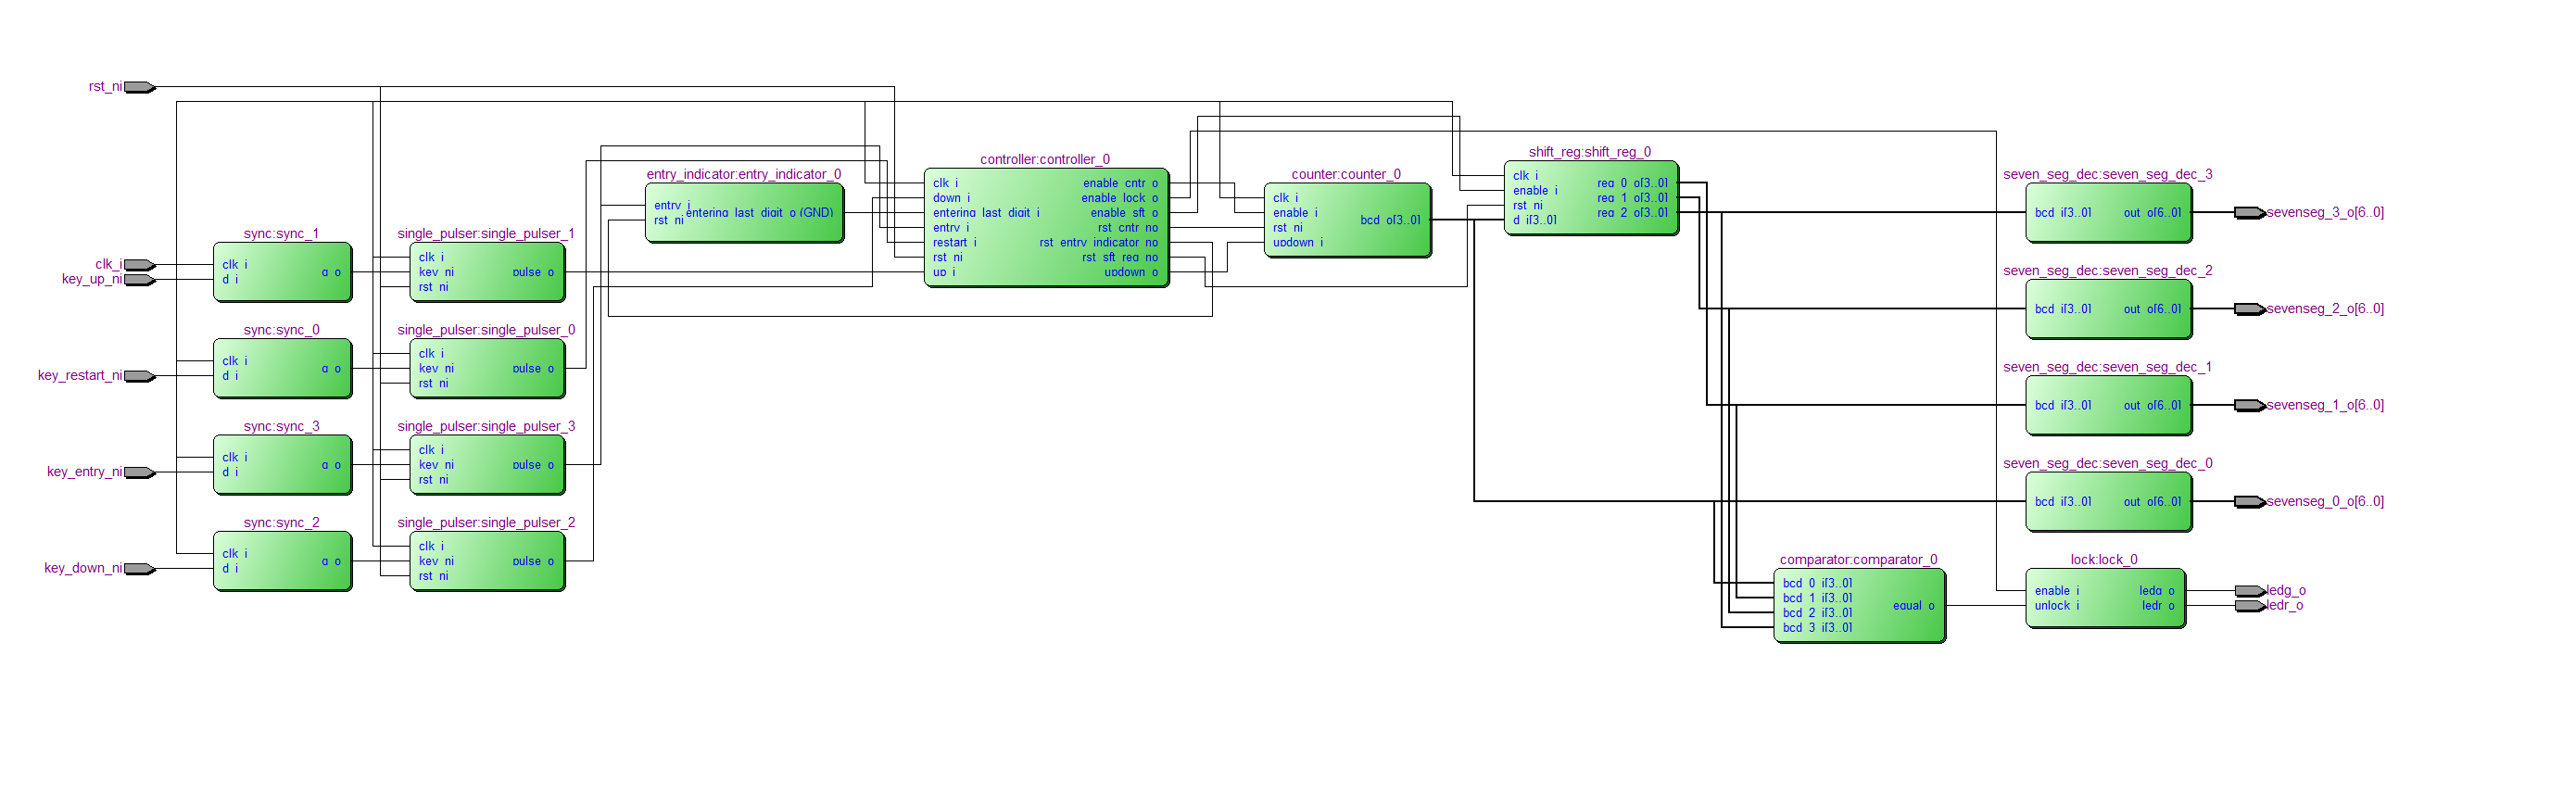
\includegraphics[width=\paperwidth]{arch_block_diagram.png}}
   \caption{Architectural block diagram for electronic safe. Please zoom in to make it clear.}
   \label{fig:arch_block_diagram}
\end{figure}

Fig.~\ref{fig:arch_block_diagram}, generated by the RTL viewer of Quartus II, is a block diagram visualisation of the architecture of the electronic safe. The left side gathers the inputs of the system and the right side gathers the outputs. The system accepts five input signals: up, down, entry, restart, and reset. All inputs go through the synchroniser and single pulser and then into the controller, except reset. The reset only connects the modules in the left half of the controller; the reset of the modules in the right half is controlled by the controller. The electronic safe uses four seven segment displays (SSD) to display the currently entered sequence of digits. The first SSD is connected directly to the output of the counter, the remaining three are connected to the three register array of the shift register. The binary coded decimal (BCD) output of the counter is also connected to the data input of the shift register. When the shift register is triggered, the input of the counter is deposited into the first register array and the data originally in each register array is moved to the next register array. The counter and shift registerr in conjunction with the controller implements the functionality of sequential inputting a digital sequence. The outputs of the counter and shift registers are fed into the comparator. The comparator outputs a matching signal to the lock. If the lock receives the matching signal, it lights up a green light-emitting diode (LED) to indicate a correct digit sequence has been given, otherwise it lights up a red LED. If the lock is not enabled, none of the LEDs are lit. The entry indicator records the number of times the entry is pressed. When the user is ready to enter the last digit, it gives the controller a flag signal. The controller uses this signal to make a state transition, which preventing the shift register from moving an extra digit.
